\documentclass[12pt,frenchb]{beamer}
\usepackage[utf8]{inputenc}
\usepackage[T1]{fontenc}
%\usepackage{ntheorem}
\usepackage{amsmath}
\usepackage{amsfonts}

\usepackage{array}

\usepackage{kpfonts}


%\pdfminorversion 7
%\pdfobjcompresslevel 3

\usepackage{tabularx}

\usepackage{pgf}
\usepackage{tikz}
\usepackage{tkz-euclide}
\usetkzobj{all}
\usetikzlibrary{patterns}


\usepackage{lastpage}

\usepackage{marginnote}

\usepackage{wrapfig}
\usepackage{babel}

\usepackage[autolanguage]{numprint}
\newcommand{\np}{\numprint}

\makeatletter

\pgfdeclarepatternformonly{mes_hachures}
{\pgfpoint{-0.1cm}{-0.1cm}}
{\pgfpoint{0.9cm}{0.5cm}}
{\pgfpoint{0.8cm}{0.4cm}}
{\pgfpathmoveto{\pgfpointorigin}
  \pgfpathlineto{\pgfpoint{0.8cm}{0.4cm}}
\pgfusepath{stroke}}

\newcommand{\R}{\mathbf{R}}
\newcommand{\N}{\mathbf{N}}
\newcommand{\Vecteur}{\overrightarrow}
\newcommand{\norme}[1]{\left\lVert #1 \right\rVert}
\newcommand{\vabs}[1]{\left\lvert #1 \right\rvert}
\newcommand{\inff}[2]{\left[#1~;~#2\right]}
\newcommand{\info}[2]{\left[#1~;~#2\right[}
\newcommand{\inof}[2]{\left]#1~;~#2\right]}
\newcommand{\inoo}[2]{\left]#1~;~#2\right[}

\makeatother


\usepackage{multicol}
\setlength{\columnseprule}{0pt}

\everymath{\displaystyle\everymath{}}

\title{Limites de fonctions}
\author{Terminale S}
\institute{Jean-Baptiste de la Salle}
\date{septembre 2017}

\begin{document}

\begin{frame}
  \maketitle
\end{frame}

\section{Limite à l'infini}

\subsection{Limite finie}

\begin{frame}
  \begin{block}{}
      \begin{definition}
        \[ \forall \varepsilon > 0,\ \exists A > 0, \forall x \geqslant A
        \implies \vabs{f(x) - \ell} \leqslant \varepsilon \]
      \end{definition}
    \end{block}
\end{frame}

\begin{frame}
  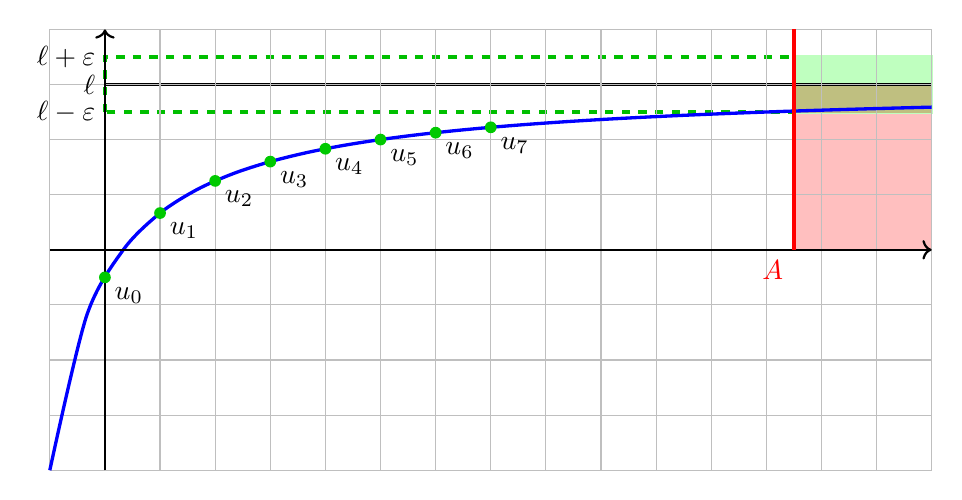
\begin{tikzpicture}[scale=0.7]
    \def\A{12.5}
    \draw [red, fill=red!25] (\A,0) rectangle (15,3) ;
    \draw [green!75!black, very thick, dashed] (0,3-0.5) rectangle (\A,3+0.5) ;
    \draw [fill,green!25, very thick] (\A,3-0.5) rectangle (15,3+0.5) ;
    \draw [fill,green!50!red!50] (\A,3-0.5) rectangle (15,3) ;
    \draw [black, very thick] (0,3) -- (15,3) ;
    \draw [thin, lightgray] (-1,-4) grid [step=1] (15,4) ;
    \draw [very thick, blue] plot [domain = -1:15,smooth]
    (\x,{(3*\x-1)/(\x+2)}) ;
    \draw [thick,->] (-1,0) -- (15,0) ;
    \draw [thick,->] (0,-4) -- (0,4) ;
    \foreach \x in {0,...,7} { \draw (\x,{(3*\x-1)/(\x+2)}) node
      [circle, fill, green!79!black, inner sep=1.5pt] {} ;
      \draw (\x,{(3*\x-1)/(\x+2)}) node [below right] {$u_{\x}$ } ;
    }
    \draw [very thick, red] (\A,0) node [below left] {$A$} -- (\A,4) ;
    \draw (0,3-0.5) node[left] {$\ell - \varepsilon$} ;
    \draw (0,3) node [left] {$\ell$} ;
    \draw (0,3+0.5) node[left] {$\ell + \varepsilon$} ;
  \end{tikzpicture}
\end{frame}

\begin{frame}

\framebox{
  \begin{minipage}{0.99\linewidth}
    Soit $f$ une fonction admettant $\ell$ pour limite en $\pm\infty$.

    La droite d'équation \alert{$y=\ell$} est une
    \alert{asymptote horizontale} à la courbe représentative de la fonction
    $\mathscr{C}_f$.
  \end{minipage}
}
\end{frame}

\begin{frame}
\end{frame}


\subsection{Limite infinie}

\begin{frame}
  \framebox{
  \begin{minipage}{0.99\linewidth}
    \begin{definition}
      \[ \forall A > 0,\exists B > 0 \forall x \geqslant B \implies f(x)
      \geqslant A \]
    \end{definition}
  \end{minipage}
}
\end{frame}

\begin{frame}
\begin{minipage}{0.99\linewidth}
  Soit $f$ une fonction admettant $+\infty$ pour limite en $+\infty$.

  S'il existe une droite d'équation \alert{$y = ax+b$} telle que
  $\lim_{x\to+\infty}f(x) - y = 0$, on dit alors que cette droite est
  une \alert{asymptote oblique} à la courbe représentative de la fonction
  $\mathscr{C}_f$.
\end{minipage}
\end{frame}


\subsection{Limite en un point}
\begin{frame}
\framebox{
  \begin{minipage}{0.99\linewidth}
    \begin{definition}
      \[ \forall \alpha > 0,\ \exists M > 0,\ \vabs{x-a} \leqslant
      \alpha \ \text{et}\ x > a\implies f(x) \geqslant M \]
    \end{definition}
    $\lim_{\substack{x\to a\\ x > a}}f(x) = +\infty$
  \end{minipage}
}

\end{frame}

\begin{frame}
\begin{center}
  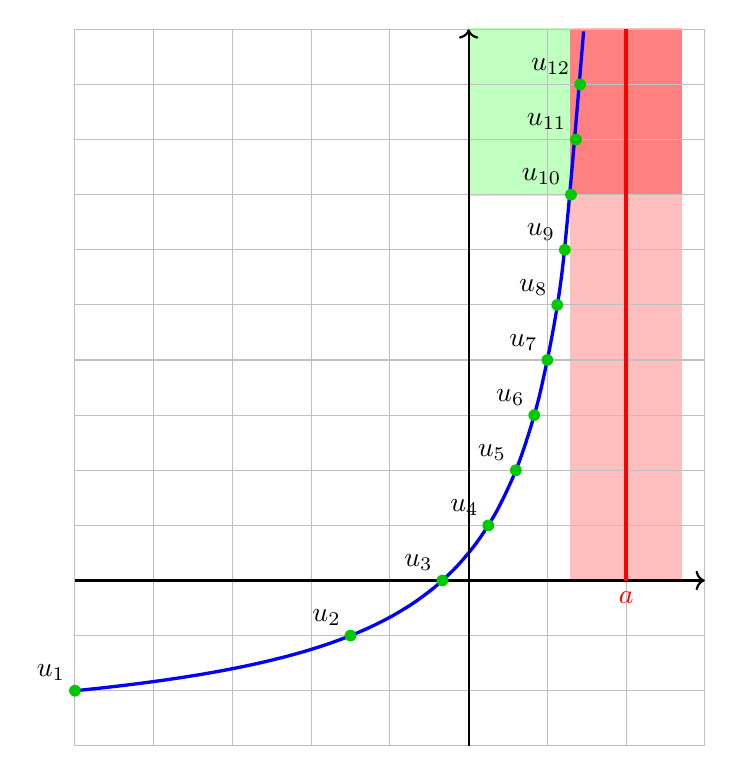
\begin{tikzpicture}[yscale=0.7]
    \def\a{2}
    \def\A{7}
    \def\e{0.7}

    \draw [red!25, thick, fill] (\a-\e,0) rectangle (\a+\e,10) ;
    \draw [green!25, thick, fill] (0,\A) rectangle (\a-\e,10) ;
    \draw [green!50,red!50, fill] (\a-\e,\A) rectangle (\a+\e,10) ;

    \draw [thin, lightgray] (-5,-3) grid [step=1] (3,10) ;
    \draw [very thick, blue] plot [domain = -1.46:5,smooth]
    (-\x,{-(3*\x-1)/(\x+2)}) ;
    \draw [thick,->] (-5,0) -- (3,0) ;
    \draw [thick,->] (0,-3) -- (0,10) ;
    \draw [red, very thick] (\a,0) node[below] {$a$} -- (\a,10) ;
    \foreach \x in {1,...,12} { \draw (2-7/\x,{-(3*(-2+7/\x)-1)/((-2+7/\x)+2)}) node
      [circle, fill, green!79!black, inner sep=1.5pt] {} ;
      \draw (-7/\x+2,{-(3*(7/\x-2)-1)/((7/\x-2)+2)}) node [above left]
      {$u_{\x}$ } ;
    }

  \end{tikzpicture}
\end{center}
\end{frame}

\begin{frame}
\framebox{
  \begin{minipage}{0.99\linewidth}
    Soit $f$ une fonction admettant $\pm\infty$ pour limite en $a$.

    La droite d'équation \alert{$ x = a$}est une
    \alert{asymptote verticale} à la courbe représentative de la fonction
    $\mathscr{C}_f$.
  \end{minipage}
}
\end{frame}

\section{Opérations sur les limites}

\subsection{Limites en $\pm\infty$}

\begin{frame}
\end{frame}

\subsection{Limites finies}

\begin{frame}
Soient $f$ et $g$ deux fonctions, définies respectivement sur
$\mathcal{D}_f$ et $\mathcal{D}_g$, avec $f(\mathcal{D}_f)\subset
\mathcal{D}_g$.

On suppose que $\lim_{x\to a}f(x) = b$, avec $a\in\mathcal{D}_f$ et
$b\in\mathcal{D}_g$.

Alors $\lim_{x\to a}g(f(x))$ existe et vaut $g(b)$ ou la limite de $g$
en $b$.
\end{frame}

\begin{frame}
  \begin{block}{remarque}
  Avec les hypothèses ci-dessus pour le domaine de définition et le
  domain image, la fonction $x\mapsto g(f(x))$ se note $(g\circ f)(x)$
  ou plus simplement $g\circ f(x)$
\end{block}
\end{frame}

\end{document}
